\chapter{METHODOLOGY}
\label{sec:chap3_metodologi}

\section*{ }
\section{Overview of the Icar System} 
The navigation system in Icar is divided into two types: the legacy navigation system using GNSS and the new navigation system that operates without GNSS. Below are block diagrams of Icar's navigation systems with and without GNSS.

\begin{figure}[H]
	\centering
	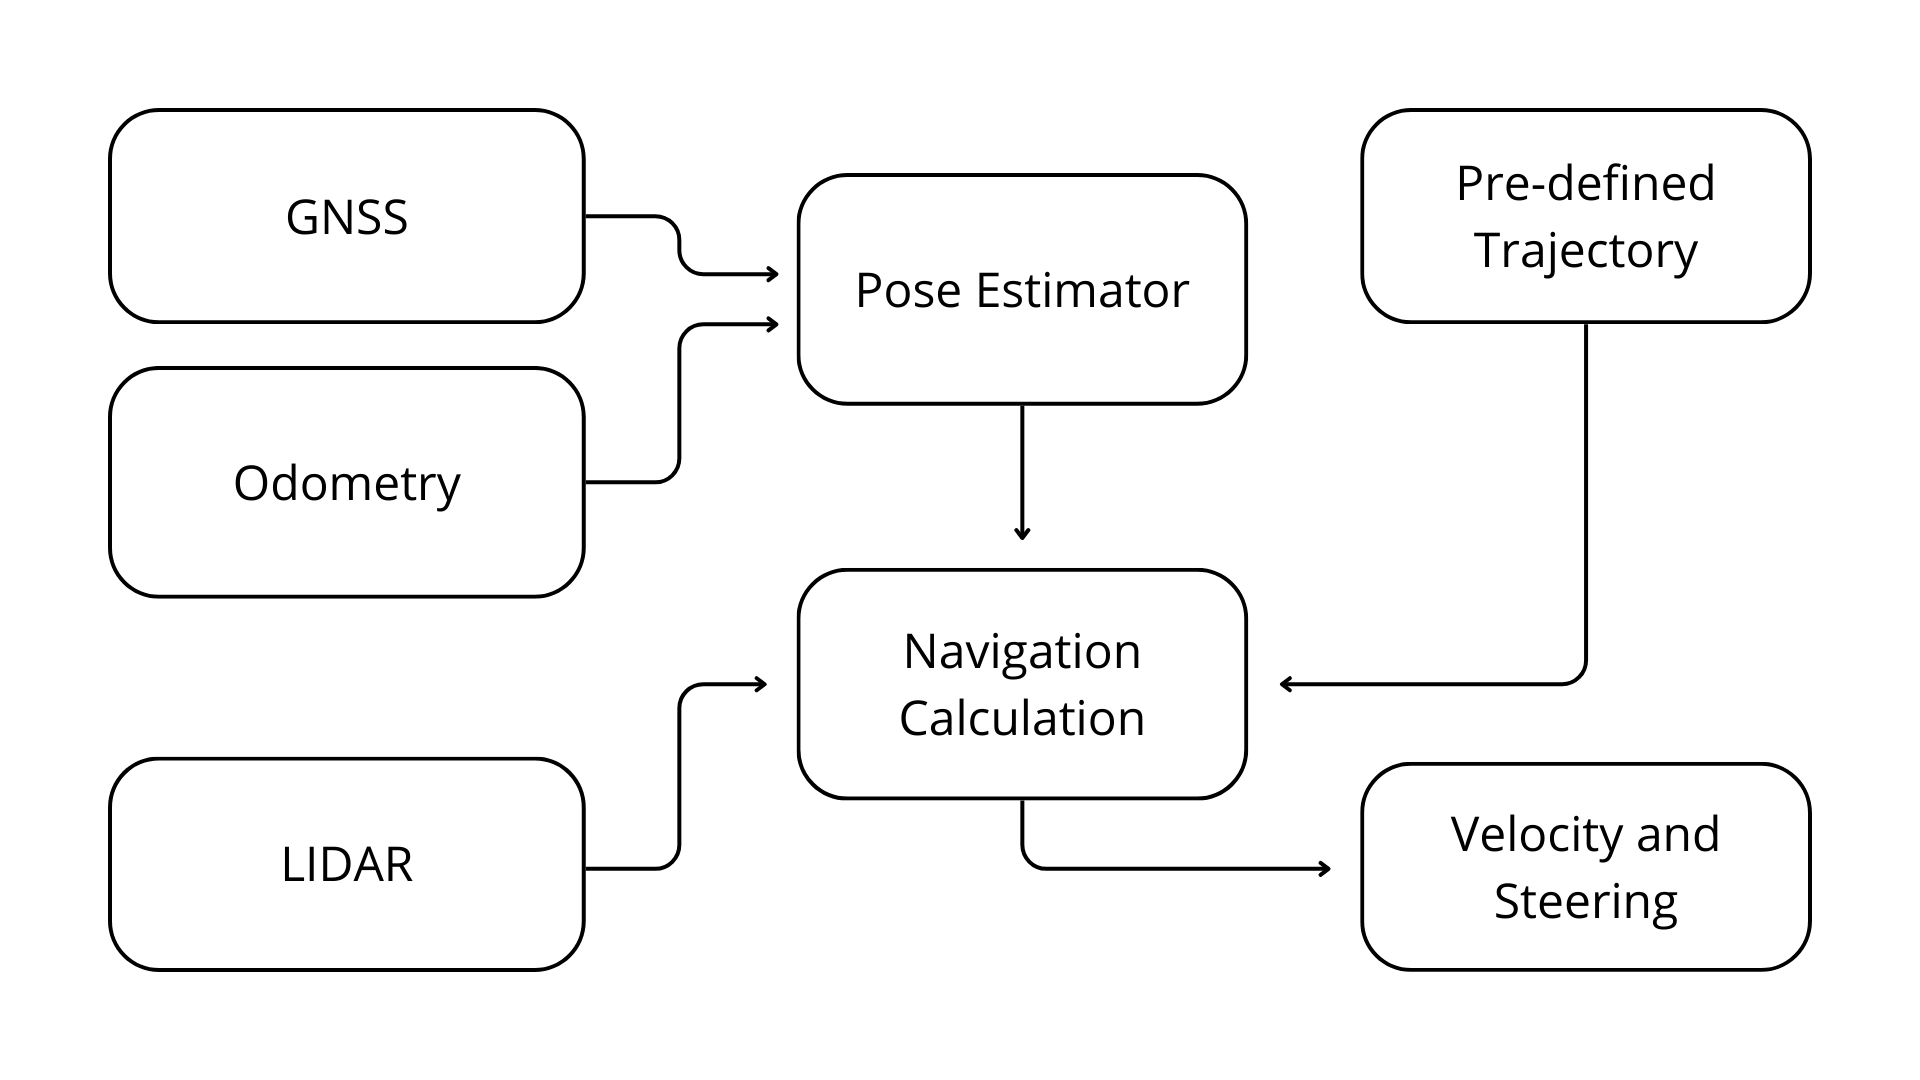
\includegraphics[width=\linewidth]{../konten/full_sys1.png}
	\caption{Block Diagram of the Legacy Icar System with GNSS}
	\label{fig:full_system}
\end{figure}
\FloatBarrier

Figure \ref{fig:full_system} illustrates the legacy Icar system, which relies on GNSS and odometry for pose estimation. The system uses a Pre-defined Trajectory to determine the target speed and steering angle using the Bicycle Model, as shown in equation~\ref{eq:bicycle_model_core}.

\begin{figure}[H]
	\centering
	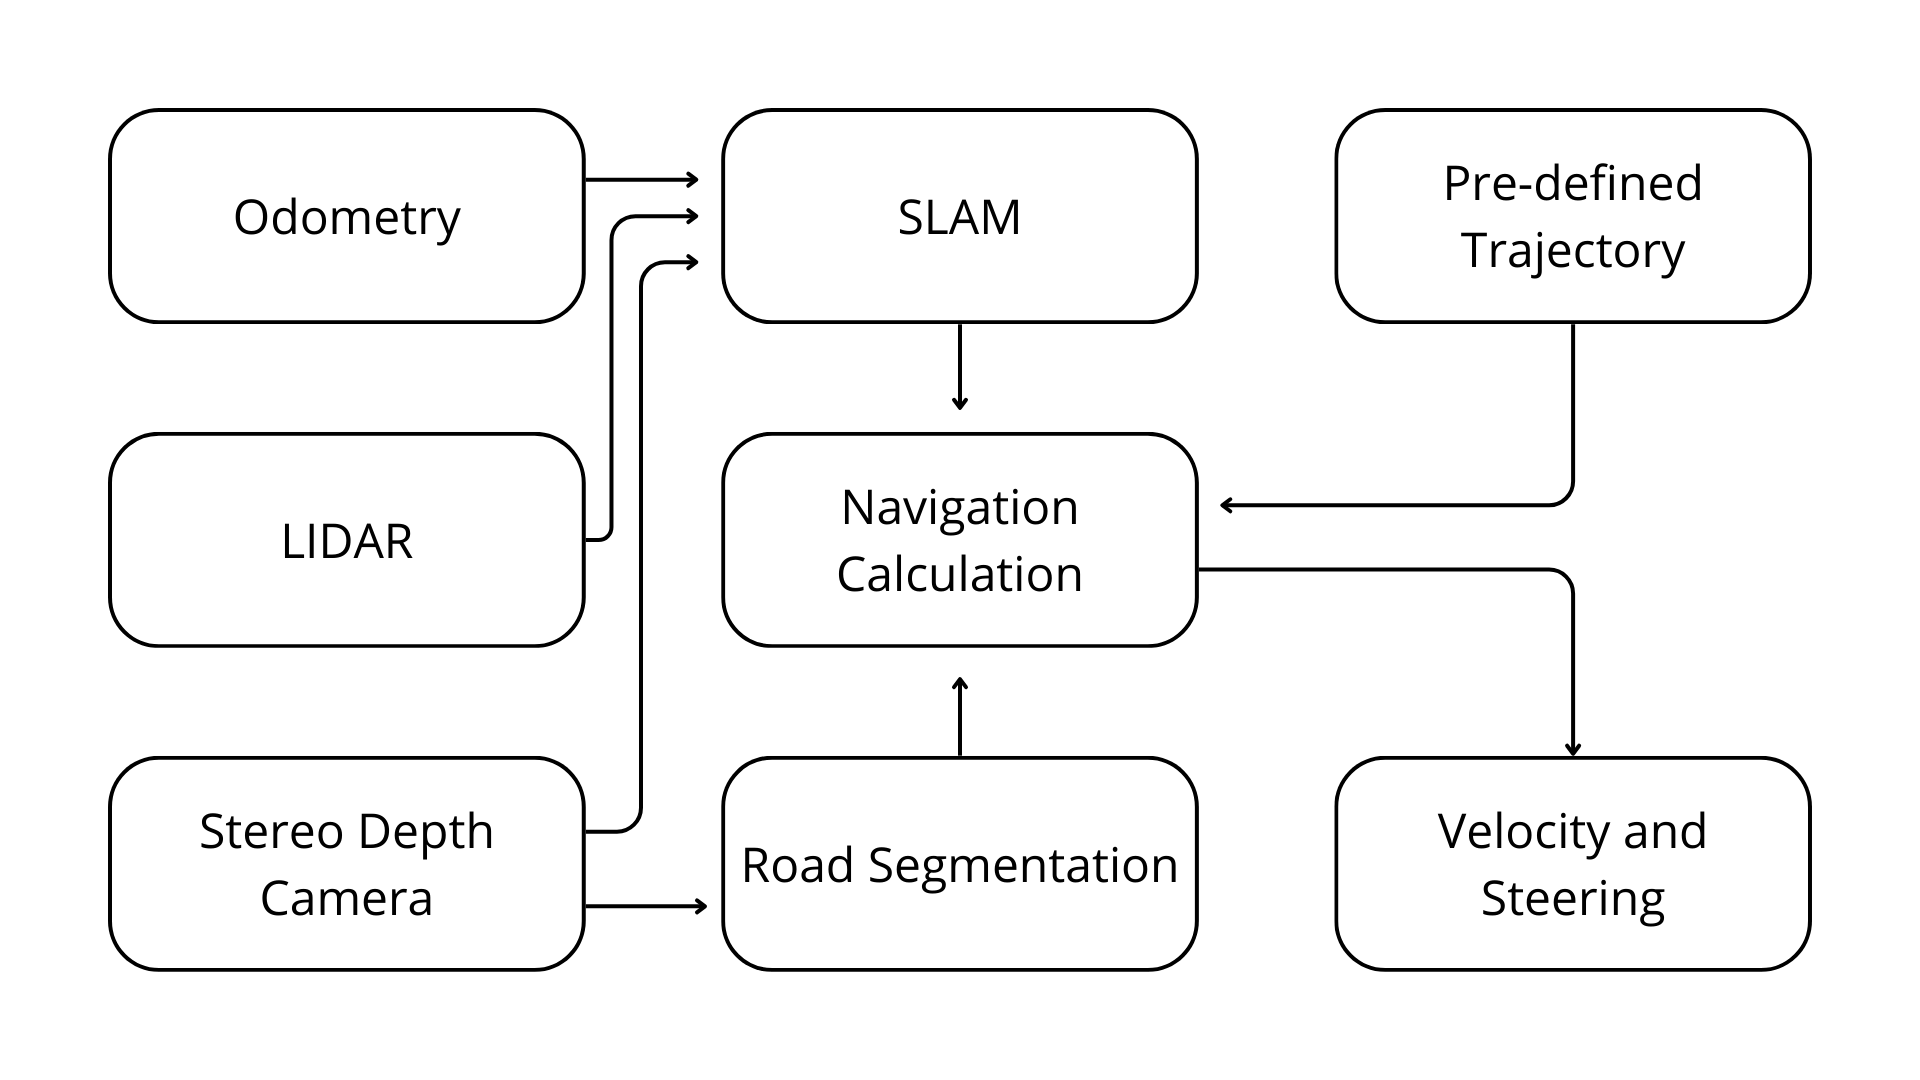
\includegraphics[width=\linewidth]{../konten/full_sys_slam1.png}
	\caption{Block Diagram of the New Icar System without GNSS}
	\label{fig:full_system_slam}
\end{figure}

Figure \ref{fig:full_system_slam} illustrates the new proposed Icar system, which does not rely on GNSS. Instead, it uses a stereo depth camera and LIDAR for pose estimation. The system also employs a Pre-defined Trajectory to determine the target speed and steering angle using the Bicycle Model, as shown in equation~\ref{eq:bicycle_model_full}. Below is the full equation for the Bicycle Model used in the new system:

\begin{equation}
	\begin{aligned}
		\Delta x &= x_{\text{waypoint}} - x_{\text{position}} \\
		\Delta y &= y_{\text{waypoint}} - y_{\text{position}} \\
		\theta_{\text{direction}} &= \tan^{-1}\left(\frac{\Delta y}{\Delta x}\right) - \theta_{\text{orientation}} \\
		v_{\text{target}} &= \min\left(\sqrt{\Delta x^2 + \Delta y^2}, \ v_{\text{max}}\right) \\
		\delta_{\text{target}} &= \tan^{-1}\left( \frac{2 \cdot L \cdot \sin(\theta_{\text{direction}})}{D_{\text{lookahead}}} \right)
		\label{eq:bicycle_model_full}
	\end{aligned}		
\end{equation}

Where $x_{\text{waypoint}}$ and $y_{\text{waypoint}}$ are the coordinates of the waypoint obtained from the Pre-defined Trajectory, $x_{\text{position}}$ and $y_{\text{position}}$ represent the vehicle's current position, $\theta_{\text{direction}}$ is the heading angle, $\theta_{\text{orientation}}$ is the current orientation, $v_{\text{target}}$ is the target velocity, $v_{\text{max}}$ is the maximum velocity, $\delta_{\text{target}}$ is the target steering angle, $L$ is the distance between the front and rear wheels, and $D_{\text{lookahead}}$ is the lookahead distance.

The primary difference between the two systems is the source of position and orientation data. The legacy system uses GNSS and odometry, while the new system uses stereo depth cameras, LIDAR, and odometry. Additionally, the new system integrates road detection to enhance navigation safety.

\section{Road Detection System}
\begin{figure}[H]
	\centering
	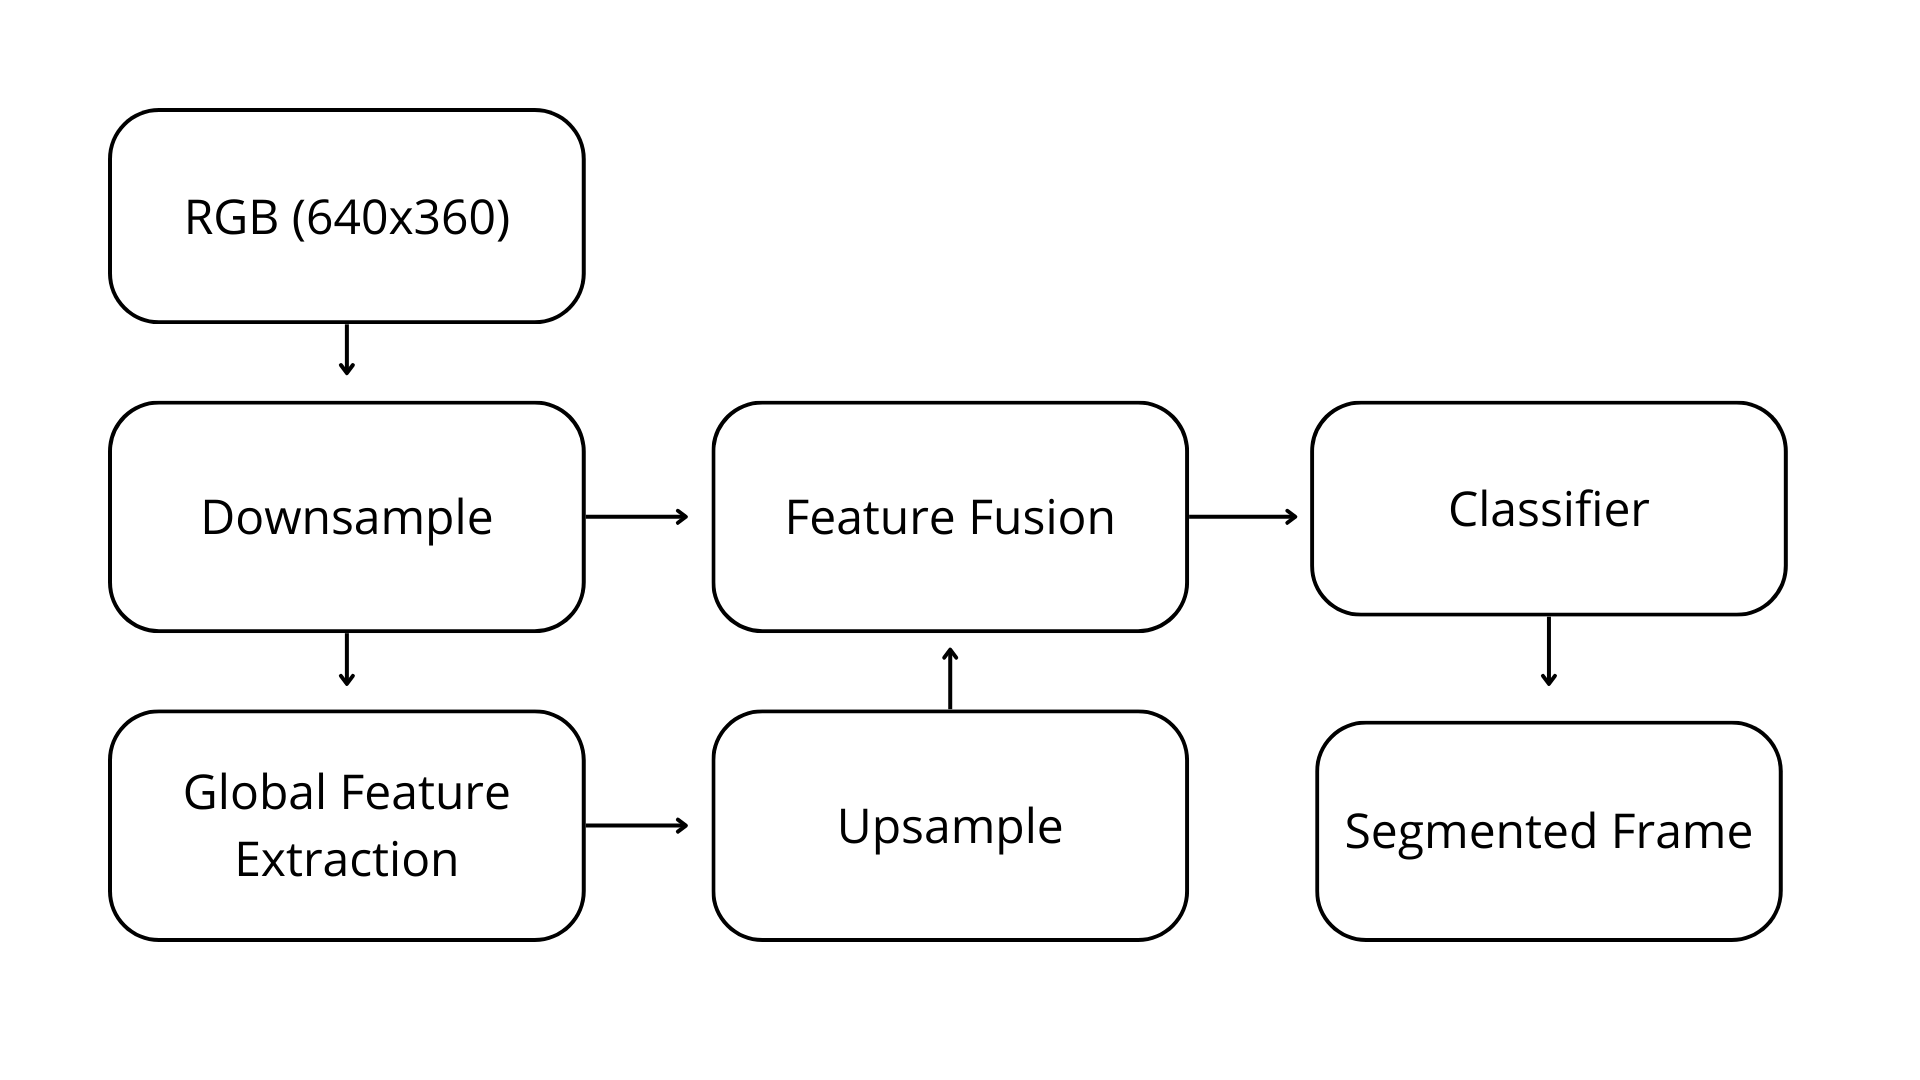
\includegraphics[width=\linewidth]{../konten/ml_sys.png}
	\caption{Block Diagram of the Machine Learning Architecture on Icar}
	\label{fig:ml_system}
\end{figure} 

From Figure \ref{fig:ml_system}, it is shown that the road detection system on Icar utilizes a machine learning architecture, specifically using Fast-SCNN \cite{ref_fast_scnn} as the core model. Its architecture differs in the convolution channels and pooling methods. The smaller convolution channels and the use of average pooling instead of pyramid pooling are intended to reduce computational load, making it suitable for real-time applications on Icar.

\subsection{Downsampling} 
In this step, the image captured by the stereo depth camera, originally a 3-channel image, is converted to 16 channels. This is achieved via three successive 3x3 convolution layers with a stride of 2: first converting 3→4 channels, then 4→8, and finally 8→16 channels. The resulting image is then split into two paths: one goes to global feature extraction, the other to feature fusion.

\subsection{Global Feature Extraction}
This stage performs a depthwise-separable convolution to extract features from the 16-channel image. This method is chosen for its computational efficiency. The result is a 24-channel image, which is passed on to the upsampling stage.

\subsection{Upsampling}
This step performs pooling using average pooling, which is lighter and faster compared to the pyramid pooling used in the original Fast-SCNN. A convolution then produces a 32-channel output, which is passed to feature fusion.

\subsection{Feature Fusion}
Here, outputs from the downsampling and global feature extraction stages are merged into a 48-channel image. Before merging, image dimensions are matched using bilinear interpolation. The merged result is passed to the classification stage.

\subsection{Classification}
In this final stage, the 48-channel image undergoes classification using ReLU, producing a 2-channel image indicating road and non-road areas. This image then proceeds to post processing.

\section{Pose and Orientation Correction System}
\begin{figure}[H]
	\centering
	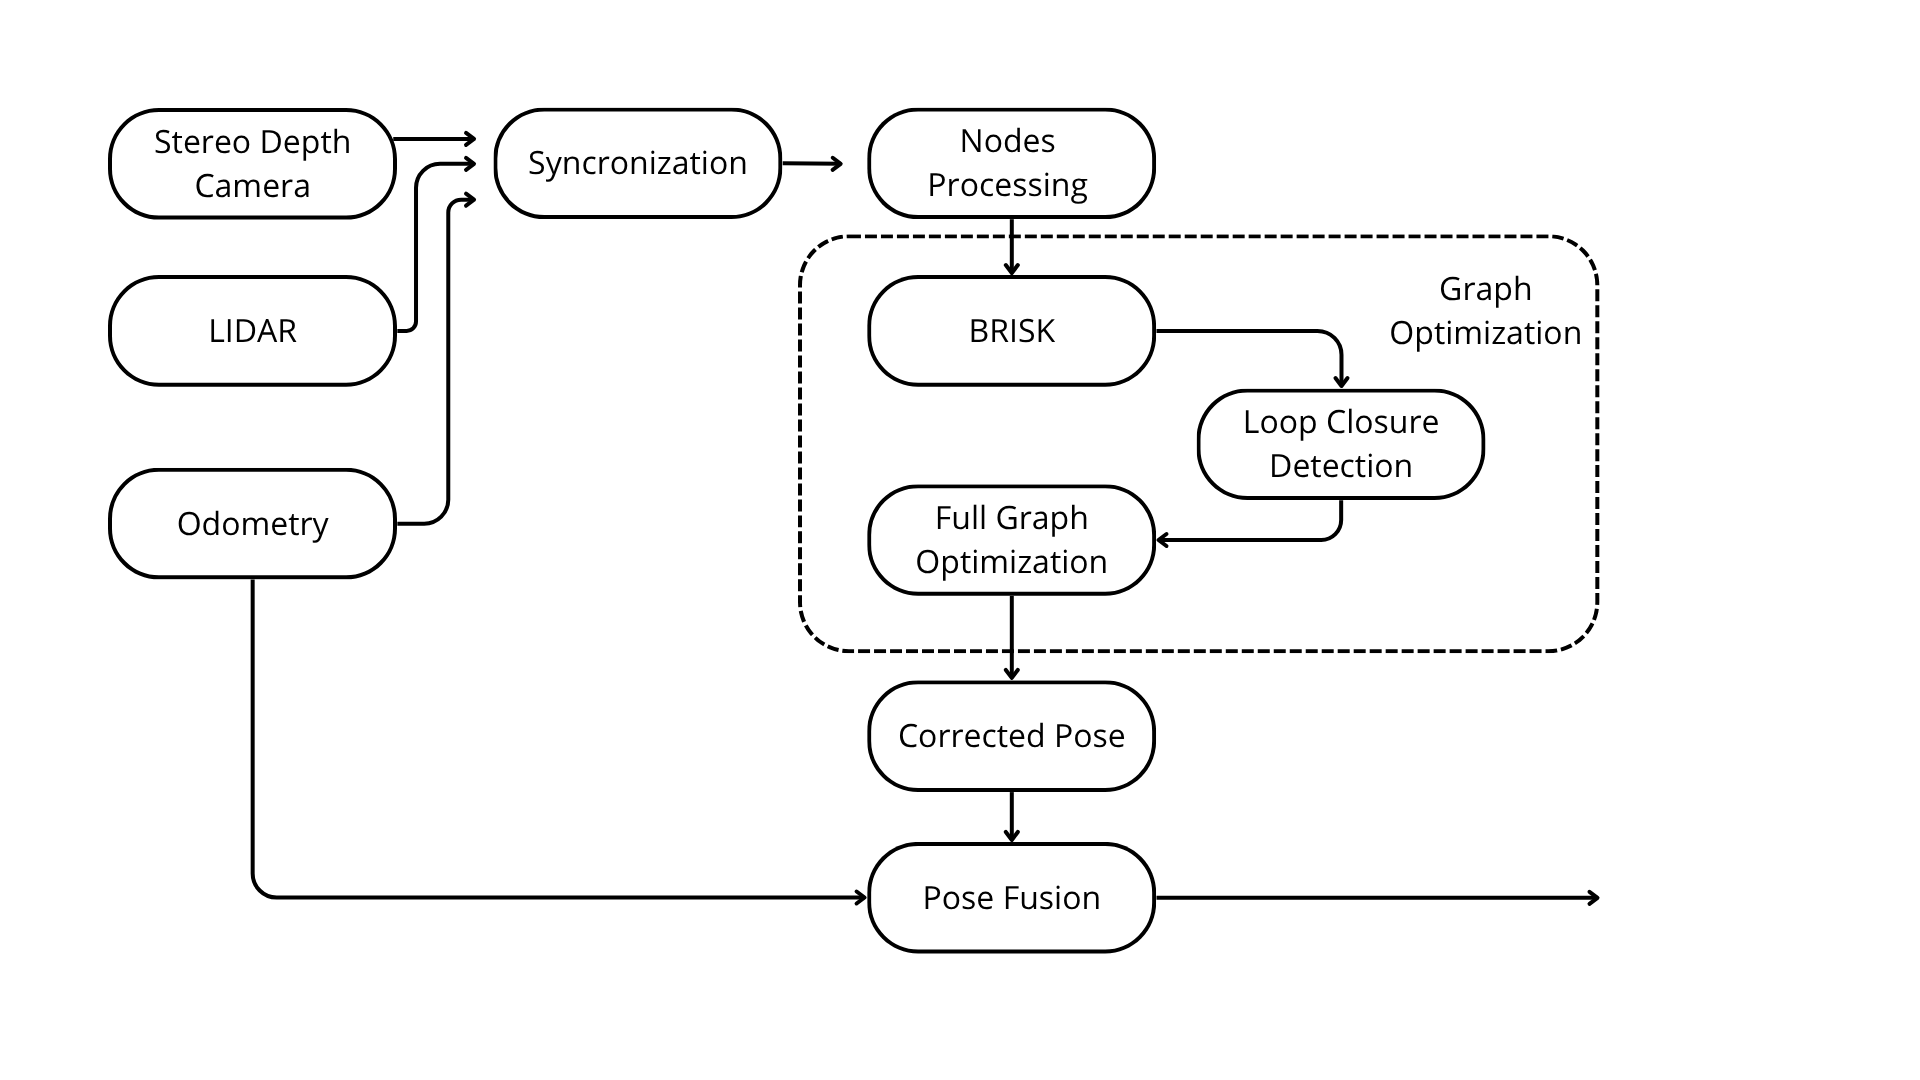
\includegraphics[width=\linewidth]{../konten/GNSS(20).png}
	\caption{Block Diagram of Pose and Orientation Correction System on Icar}
	\label{fig:slam_system}
\end{figure} 

From Figure \ref{fig:slam_system}, the pose correction system consists of four main processes: data synchronization, nodes processing, graph optimization, and pose fusion.

\subsection{Data Synchronization} 
This initial step synchronizes data from the stereo depth camera and odometry based on timestamps to ensure aligned data for further processing.

\subsection{Nodes Processing}
This initiates the graph optimization process. Nodes represent vehicle poses and keypoints from stereo depth camera and LIDAR. There are two modes:
- In mapping mode, new nodes are continuously added.
- In localization mode, existing nodes are used without adding new ones.

\subsection{Graph Optimization} 
This is the core component, using the GTSAM library. It starts finding loop closure by detecting revisited nodes, which are nodes that have been previously visited by the vehicle. The algorithm to do image matching is using BRISK. After the hypothesis of loop closure has gained, the next step is doing a full graph optimization using GTSAM, the GTSAM will minimize the error between the current pose and the previous pose, as well as the error between the current pose and the loop closure hypothesis. The result is a corrected pose of the vehicle.

\subsection{Pose Fusion} 
The final step combines poses from graph optimization and odometry using a Kalman Filter, resulting in more accurate pose estimation than using odometry alone. Using the differential data from Odometry (Wheel encoder and IMU) combined with estimated pose that coming from Graph Optimization, the system can correct the pose and orientation of Icar.

\section{Icar Navigation System with Road Detection and Graph-Based SLAM} 
\begin{figure}[H]
	\centering
	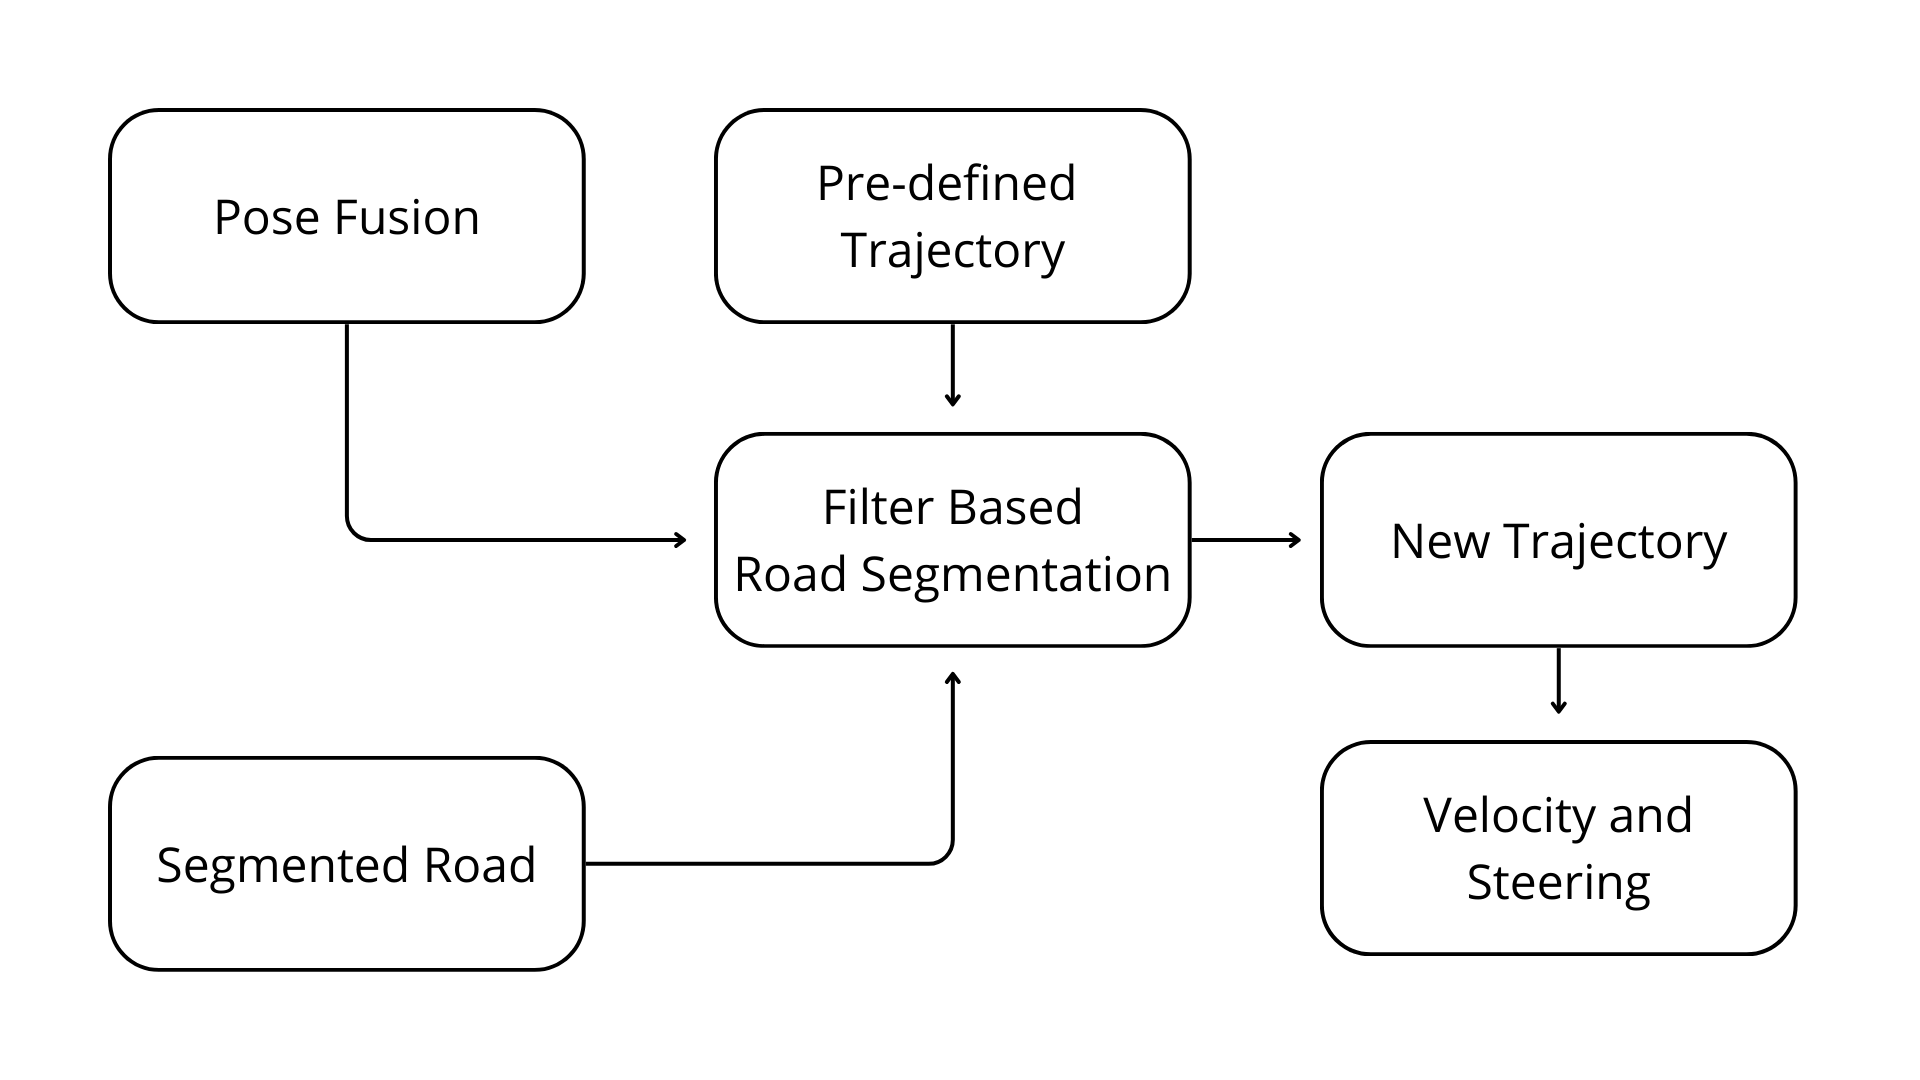
\includegraphics[width=\linewidth]{../konten/nav_new_sys3.png}
	\caption{Block Diagram of Icar Navigation System with Road Detection and Graph-Based SLAM}
	\label{fig:nav_new_system}
\end{figure} 

This diagram expands upon Figure \ref{fig:full_system_slam}, showing how the segmented road image from Figure \ref{fig:ml_system} and the pose data from Figure \ref{fig:slam_system} are integrated into a unified and improved navigation system.

\par  
The first step selects waypoints based on current pose (from graph-based SLAM) and the pre-defined trajectory. These waypoints are overlaid on the road segmentation image.

\par   
Next, a check is performed using a bitwise AND operation to determine if all waypoints lie within the road area. If so, the selected waypoints are used as the new trajectory.

\par  
If any waypoint lies outside the road, a new trajectory is generated using the image’s center of mass, converted into vehicle coordinates. A straight line is then created from the current position to the center of mass.

\par 
This new trajectory is then used for vehicle navigation. The vehicle follows it using the Bicycle Model as defined in Equation \ref{eq:bicycle_model_full} to calculate target speed and steering angle.
